\documentclass[aspectratio=169]{beamer}

\usepackage{default}
\usepackage[utf8]{inputenc}
\usepackage[T1]{fontenc}
\usepackage[spanish]{babel}
\usepackage{graphicx}
\usepackage{wrapfig}
\usepackage{listings}
\usepackage{lipsum}

% ==================================================================================
% Tipos
% ==================================================================================
\usepackage[light,condensed,math]{kurier}


% ==================================================================================
%  Símbolos matemáticos
% ==================================================================================

\usepackage{amsmath}
\usepackage{amsfonts}
\usepackage{amsthm}

\def\N{\ensuremath{\mathbb{N}}}
\def\Z{\ensuremath{\mathbb{Z}}}
\def\Q{\ensuremath{\mathbb{Q}}}
\def\R{\ensuremath{\mathbb{R}}}
\def\C{\ensuremath{\mathbb{C}}}


% ==================================================================================
%  Colores
% ==================================================================================

\usepackage[]{xcolor}

\definecolor{azulUCA}{cmyk}{1.00, 0.00, 0.00, 0.51}
\definecolor{naranjaUCA}{cmyk}{0.00, 0.51, 1.00, 0.00}
\definecolor{grisUCA}{cmyk}{0.00, 0.00, 0.00, 0.65}
\definecolor{charcoal}{rgb}{0.21, 0.27, 0.31}
\definecolor{darkjose}{HTML}{4a4a4a}

% ==================================================================================
%  Algunos diseños
% ==================================================================================
\usepackage{epigraph}

\newcommand{\citainicial}[1]{
	\raya
	\begin{quotation}
		\color{charcoal}{\textit{#1}}
	\end{quotation}
	\raya
}

\def\raya{
	\par \hbox to
	\linewidth{\hss \vrule width \textwidth height 0.2pt depth 0.5pt}
	\par}

\makeatletter

\newcommand{\seccion}[1]{
	\section*{\color{azulUCA}{#1}}
}

\newcommand{\subseccion}[1]{
	\subsection*{\color{naranjaUCA}{#1}}
}

\usepackage[theorems,breakable]{tcolorbox}

\tcbuselibrary{theorems}

\newtcbtheorem{problema}{Problema}%
{
	colback=azulUCA!5,
	colframe=azulUCA,
	fonttitle=\bfseries
}{pr}

\newtcbtheorem{formulacion}{Formulación}%
{
	colback=naranjaUCA!5,
	colframe=naranjaUCA,
	fonttitle=\bfseries
}{for}

\newtcbtheorem{autores}{Autores}%
{
	colback=charcoal!5,
	colframe=charcoal,
	fonttitle=\bfseries
}{aut}

\addtobeamertemplate{background canvas}{\transboxin}{}
% ==================================================================================
%  Definiciones
% ==================================================================================
\title{Teoria de colas}
\date{}
\begin{document}

\begin{frame}
	\titlepage
	\begin{center}
		\href{http://creativecommons.org/licenses/by-sa/3.0/es/}{\includegraphics[width=4em]{cc-by-sa}}
	\end{center}
\end{frame}


\begin{frame}
	\centering \LARGE \color{naranjaUCA} Introducción
\end{frame}
\begin{frame}{¿Qué es un proceso estocástico?}
	
\begin{itemize}
	\item Un \textbf{proceso estocástico }$\lbrace X_t, t \in T \rbrace$ es una colección de variables aleatorias definidas sobre el mismo espacio de probabilidad ($\Omega,S,P$). El conjunto $T$ se llama índice del proceso. Si $T$ es numerable diremos que el proceso estocástico es de tiempo discreto ($T=\lbrace 0,1,2,... \rbrace$) y si es continuo diremos que estamos ante un proceso estocástico de tiempo continuo ($T=\lbrace t, t\geq 0 \rbrace$).
	
\end{itemize}

\end{frame}
\begin{frame}{¿Qué es una cadena de Markov?}
	\begin{itemize}
		\item Sea $\lbrace X_n, n=0,1,2,...\rbrace$ un proceso estocástico de tiempo discreto. Suponemos que en cualquier instante, el proceso toma un número finito o numerable de valores (llamados estados del proceso).
		Un proceso estocástico de tiempo discreto es una \textbf{Cadena de Markov}, si para $t$=0,1,2,... y los estados $i_0, i_1,...,i_{n-1},i,j$:
		\pause
		$$
		P(X_{n+1}=j|X_n=i, X_{n-1}=i_{n-1},...,X_1=i_1, X_0=i_0)=
		$$ $$P(X_{n+1}=j|X_n=i_n)=p_{ij}
		$$
	\end{itemize}
\end{frame}

\begin{frame}{Ejemplo cadena de Markov}
	
	$$ 	\begin{array}{cccc}
	& 1 ~~ & 2 ~~ &  3
	\end{array}
	$$
	$$
	\begin{array}{c}
	1 \\ 2 \\ 3
	\end{array}
	\left(
	\begin{array}{ccc}
	1/3 & 1/3 & 1/3 \\
	1/3 & 0 & 2/3 \\
	1/2 & 1/2 & 0 \\
	\end{array}
	\right)
	$$
	
	\pause
	%\begin{figure*}[h]
		\centering
		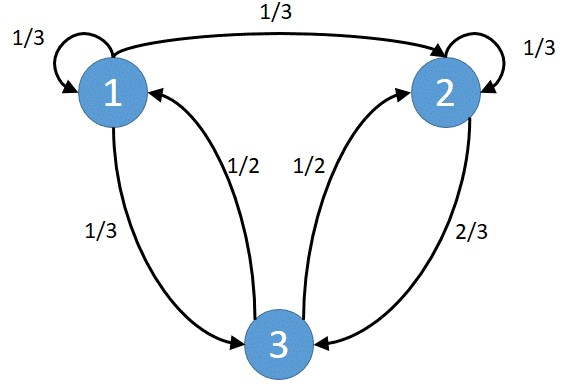
\includegraphics[width=0.4\textwidth]{grafo1}
		\label{grf1}
	%\end{figure*}
\end{frame}

\begin{frame}{¿Cuál es la probabilidad de estar en el estado $j$ después de n periodos?}
	$$
	p_{ij}^n=P(X_{m+n}=j|X_m)=P(X_n=j|X_0=i)
	$$
\end{frame}

\begin{frame}{Probabilidad de estado estable}
	Cuando $n$ es suficientemente grande
	$$
	p_{ij}^{n+1}\cong p_{ij}^n
	$$
	\pause
	En el límite
	$$
	lim ~  p_{ij}^n = \pi_j 
	$$
\end{frame}

\begin{frame}
	\centering \LARGE \color{naranjaUCA} Procesos de nacimientos y muerte
\end{frame}

\begin{frame}{Procesos de nacimientos y muerte}
	\begin{center}
		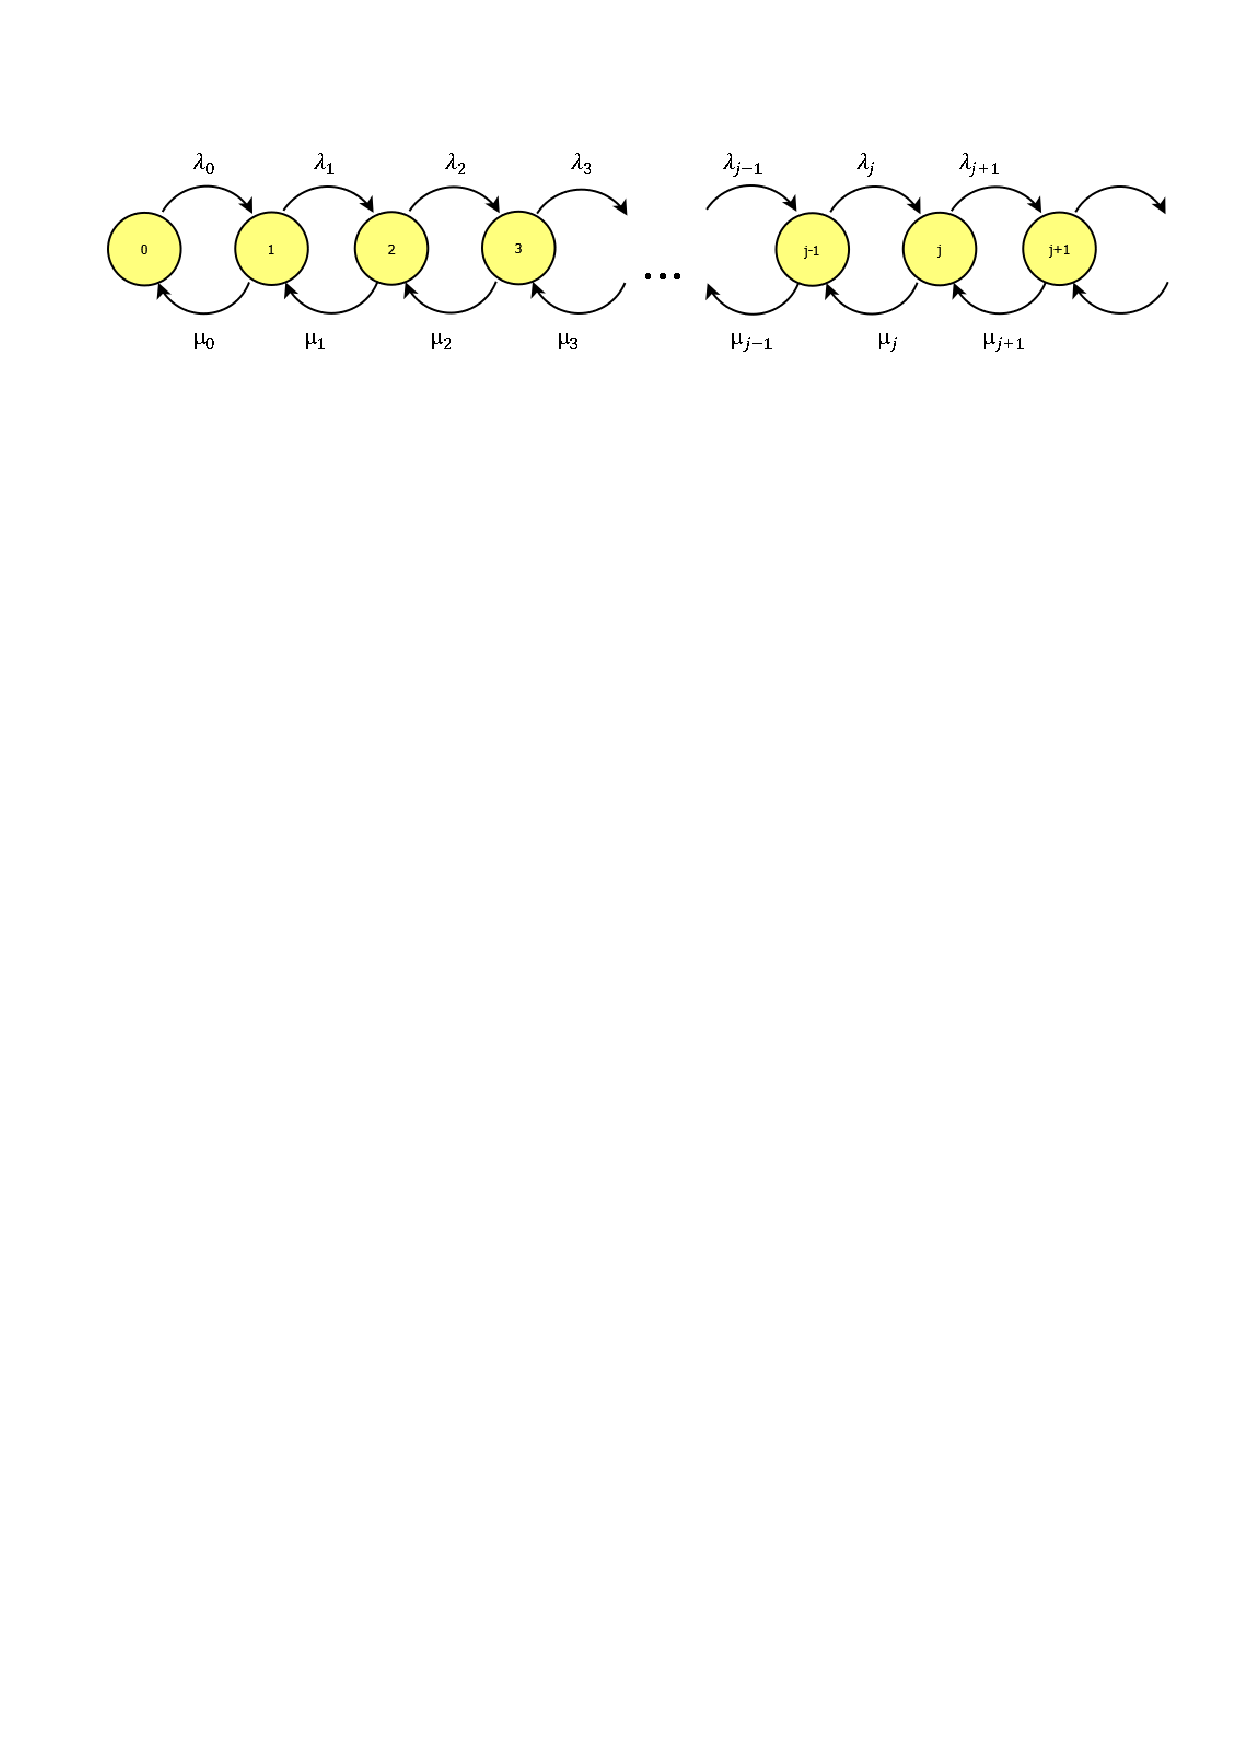
\includegraphics[trim = 10mm 220mm 10mm 25mm, clip,width=0.9\linewidth]{diagramatasa}
	\end{center}
	\pause
	Consideramos $p_{ij}^n$ la probabilidad de que, habiendo $i$ personas en el sistema, después de $n$ pasos haya $j$ personas. \\
	A partir de ahora supondremos que estamos en un estado estable.

\end{frame}
\begin{frame}{Leyes de movimientos}
	\begin{itemize}
		
		\item $P$(1 nacimiento entre $(t, t+h)$)=$\lambda_j h +o(h)$.\\
		El estado se incrementa en 1, esto es, $X(t+h)=j+1$.

		\item $P$(1 muerte entre $(t, t+h)$)=$\mu_j h +o(h)$.\\
		El estado se disminuye en 1, esto es, $X(t+h)=j-1$.
		
		\item Los nacimientos y muertes son independientes.
		
		
	\end{itemize} 

\end{frame}

\begin{frame}{Cáculo $\pi_{ij}$}
	Para $h$ pequeña: \pause
	
	\begin{equation*}
	\begin{split}
	p_{ij}(t+h)= p_{i,j-1}(t)P(\textrm{1 nacimiento en } (t,t+h))+\\
	+ p_{i,j+1}(t)P(\textrm{1 muerte en }(t,t+h))+\\
	+ p_{ij}(t)P(\textrm{ningún nacimiento ni muerte en }(t,t+h))
	\end{split}
	\end{equation*}
	\pause
	
	\begin{equation*}
	\begin{split}
	p_{ij}(t+h)= p_{i,j-1}(t)(\lambda_{j-1}h + o(h))+\\
	+ p_{i,j+1}(t)(\mu_{j+1}h + o(h))+\\
	+ p_{ij}(t)(1-\lambda_{j}h - \mu_{j}h + o(h) )
	\end{split}
	\end{equation*}
	
\end{frame}

\begin{frame}
	Reagrupando, diviendo entre $h$, tomando límite cuando $h \longrightarrow 0$:
	\pause
	\begin{equation*}
	p_{ij}'(t)= \lambda_{j-1} p_{i,j-1}(t) + \mu_{j+1}  p_{i,j+1}(t) - \lambda_j  p_{ij}(t) - \mu_{j} p_{ij}(t)
	\end{equation*}
	\pause
	Sustituyendo ahora las probabilidades de estado estable y reagrupando:
	\pause
	\begin{equation*}
	\lambda_{j-1} \pi_{j-1} + \mu_{j+1}  \pi_{j+1} = \pi_j(\lambda_j + \mu_j) \qquad (j= 1,2,...) \label{eq1}
	\end{equation*} 
	\pause
	Para $j=0$
	\pause
	\begin{block}{Ecuaciones de balance de flujo}
		\begin{equation*}
		\mu_1 \pi_1 = \pi_0 \lambda_0
		\label{eq2}
		\end{equation*}
	\end{block}
\end{frame}

\begin{frame}{Cálculo de los $\pi_{ij}$}
	Utilizando las hecuaciones de valance
\end{frame}

\begin{frame}{Cálculo de los $\pi_{ij}$}
	Utilizando las ecuaciones de balance 
	\begin{equation*}
	\pi_1=\frac{\pi_0 \lambda_0}{\mu_1}
	\label{eq3}
	\end{equation*}
	
	\pause
	Al sustituirlo en las ecuaciones de balance: para $j=1$ y despejando $\pi_2$ tenemos
	
	\begin{equation*}
	\pi_2=\frac{\pi_0(\lambda_0 \lambda_1)}{\mu_1 \mu_2}
	\label{eq4}
	\end{equation*}
	
	\pause
	Procediendo análogamente para $j=3,4,..$ se tiene que
	
	\begin{equation*}
	\pi_j=\pi_0 c_j
	\label{eq5}
	\end{equation*}
	
	$c_j=\dfrac{\lambda_0 \lambda_1 \cdots \lambda_{j-1}}{\mu_1 \mu_2 \cdots \mu_j}$
\end{frame}

\begin{frame}{Cálculo de los $\pi_{ij}$}
	Usando que \begin{equation*}
	\sum_{j=0}^{\infty}\pi_j=1 
	\label{eq6}
	\end{equation*}
	
	\pause
	Tenemos:
	\begin{equation*}
	\pi_0=\dfrac{1}{1+\sum_{j=1}^{\infty} c_j}
	\label{eq6}
	\end{equation*}
	\pause
	Se puede demostrar que si:
	$$
	\sum_{j=1}^{\infty} c_j = \infty $$
	Entonces el sistema no existe una distribución de estado estable.
\end{frame}


\begin{frame}
	\centering \LARGE \color{naranjaUCA} Introducción al sistema de líneas de espera
\end{frame}
\begin{frame}{Introducción al sistema de líneas de espera}
	\begin{block}{Procesos de llegadas}
		Definimos las llegadas como los clientes que llegan. Para este tipo de problemas solemos asumir que, en un instante dado, no puede haber más de una llegada.
	\end{block}
	\pause
	Normalmente, un proceso de llegadas no se ve afectado por el número de clientes que presenta el sistema, excepto en algunos casos:
	\begin{itemize}
		\pause
		\item \textbf{Modelos de origen finito:} Las llegadas están sacadas de una población pequeña.
		\pause
		\item \textbf{Razón:} La razón a la cual llegan los clientes a cierta instalación disminuye cuando ésta se llena.
	\end{itemize} 
\end{frame}


\begin{frame}{Introducción al sistema de líneas de espera}
	\begin{block}{Procesos de salida}
		Una salida sucede cuando un cliente ha sido servido.
	\end{block}
	
	\pause
	Existen dos tipos de servidores:
	\begin{itemize}
		\pause
		\item \textbf{Servidores en paralelo:} Si todos ofrecen el mismo tipo de servicio y un cliente sólo requiere pasar por un servidor para completar el servicio.
		\pause
		\item\textbf{Servidores en serie:} Cuando un cliente debe pasar por varios servidores antes de terminar el servicio.
	\end{itemize}
\end{frame}

\begin{frame}{Introducción al sistema de líneas de espera}
	\begin{block}{Disciplinas de líneas de espera}
		La disciplina explica el método usado para determinar el orden en el que se atiende a los clientes.
	\end{block}
	
	\pause
	\begin{itemize}
		\item \textbf{FCFS:} Se atiende a los clientes según el orden en que llegan.
		\pause
		\item\textbf{LCFS:} Las llegadas más recientes son los primeros clientes en entrar al servicio.
		\pause
		\item\textbf{SIRO:} El siguiente cliente en pasar al servidor es elegido en forma aleatoria.
		\pause
		\item\textbf{Prioridad en las colas:} Clasifica cada llegada en una categoría. Cada categoría recibe luego un nivel de prioridad, y dentro de cada nivel de prioridad, los clientes entran en el servicio siguiendo FCFS.
		
	\end{itemize}
\end{frame}

\begin{frame}
	\centering \LARGE \color{naranjaUCA} Kendall-Lee
\end{frame}
\begin{frame}{Kendall-Lee}
Cada sistema de líneas de espera se describe mediante seis características:
1/2/3/4/5/6
\\
		La primera especifica la naturaleza del proceso de llegada. Se utilizan las abreviaturas siguientes:
		\pause
		\begin{itemize}
			\item M=Los tiempos entre llegadas son variables aleatorias independientes e idénticamente distribuidas (iid) cuya distribución es exponencial.
			\pause
			\item D= Los tiempos entre llegadas son iid y deterministas. \pause
			\item $E_k$=Los tiempos entre llegadas son Erlangs iid con parámetro de forma k.
			\pause
			\item GI=Los tiempos entre llegadas son iid y están regidos por alguna distribución general.
			\pause
		\end{itemize}

\end{frame}

\begin{frame}{Kendall-Lee}
	
	La segunda característica especifica la naturaleza de los tiempos de servicio.
	\pause
	\\
	La tercera característica es la cantidad de servidores en paralelo. 
	\pause
	\\ La cuarta característica es la disciplina de líneas de espera.
	\pause
	\\	La quinta denota la capacidad del sistema.
	\\
	\pause
	
	La sexta es el tamaño de la población de donde se extraen los clientes.
\end{frame}



\begin{frame}
	\centering \LARGE \color{naranjaUCA} Fórmulas de Little
\end{frame}
\begin{frame}\frametitle{Fórmulas de Little}
	\pause
	\begin{itemize}
		\item $\lambda$=ratio de entrada de clientes por unidad de tiempo \pause
		\item$L$= n\'umero medio de clientes en el sistema \pause
		\item$L_q$= n\'umero medio de clientes en la cola \pause
		\item$L_s$=n\'umero medio de clientes siendo servidos \pause
		\item$W$= tiempo medio que un cliente pasa en el sistema \pause
		\item$W_q$=tiempo medio que un cliente pasa en la cola \pause
		\item$W_s$= tiempo medio que un cliente tarda en ser servido \pause
	\end{itemize}
\end{frame}

\begin{frame}\frametitle{Fórmulas de Little}
	
	Para cualquier sistema de colas en el que exista el estado estable, se tienen las siguientes relaciones:
	 \pause
	\begin{itemize}
		\item $L=\lambda W$
		\pause
		\item$L_q=\lambda W_q$
		\pause
		\item$L_s=\lambda W_s$
		\pause
	\end{itemize}
\end{frame}


\begin{frame}
	\centering \LARGE \color{naranjaUCA} Modelo de cola M/M/1
\end{frame}
\begin{frame}{M/M/1}
	   Este modelo puede ser representado como un proceso  de nacimiento-muerte con los siguientes parámetros: \pause
		$$\begin{array}{cc}
		\lambda_j=\lambda & (j=0,1,...)\\ \pause
		\mu_0=0 &  \\ \pause
		\mu_j=\mu &  (j=1,2,...)\\
		\end{array}$$ \pause
		Sabiendo que $\pi_j=\pi_0 c_j$ tenemos: \pause
			\begin{center}
				$\pi_1=\pi_0\rho, \qquad \pi_2=\pi_0\rho, \qquad...,\qquad\pi_j=\pi_0\rho$
				
			\end{center} \pause
			\hspace{0.5cm}Donde $\rho=\frac{\lambda}{\mu}$
\end{frame}
\begin{frame}{M/M/1}
		Sabemos que 
			\begin{center}
			$1=\sum_{j=0}^{\infty}\pi_j=\pi_0(1+ \rho +\rho^2+\rho^3+...)$
		\end{center} \pause
		Asumiendo que $0\neq\rho<1$, llegamos a \pause
		\\ 	\begin{center}
			$\pi_0=1-\rho$
		\end{center}
		\pause
		Por lo tanto: \pause
		\begin{center}
			$\pi_j=\rho^j(1-\rho)$
		\end{center}
\end{frame}
\begin{frame}{M/M/1}
	\begin{block}{Cálculo de L}
	\begin{itemize}
		\item
		\begin{equation}
		L=(1-\rho)\frac{\rho}{(1-\rho)^2}=\frac{\rho}{1-\rho}=\frac{\lambda}{\mu-\lambda}
		\end{equation} \pause
		\item
			\begin{center}
				$L_s=0\pi_0+1(\pi_1+\pi_2+...)=1-\pi_0=1-(1-\rho)=\rho$
			\end{center} \pause
			\item
				\begin{center}
					$L_q=L-L_s=\frac{\rho^2}{1-\rho}$
				\end{center}
				\end{itemize}
		
	\end{block}
	
\end{frame}
\begin{frame}{M/M/1}

		\begin{block}{Cálculo de W}
		Usando las fórmulas de Little: \pause
		\begin{itemize}
			\item $W=\frac{L}{\lambda}=\frac{1}{\mu-\lambda}$ \pause
			\item $W_q=\frac{L_q}{\lambda}=\frac{\lambda}{\mu(\mu-\lambda)}$ \pause
			\item$W_s=\frac{L_s}{\lambda}=\frac{1}{\mu}$
		\end{itemize}
		\end{block}
\end{frame}

\begin{frame}
	\centering \LARGE \color{naranjaUCA} Modelo de cola M/M/1/c
			\begin{center}
				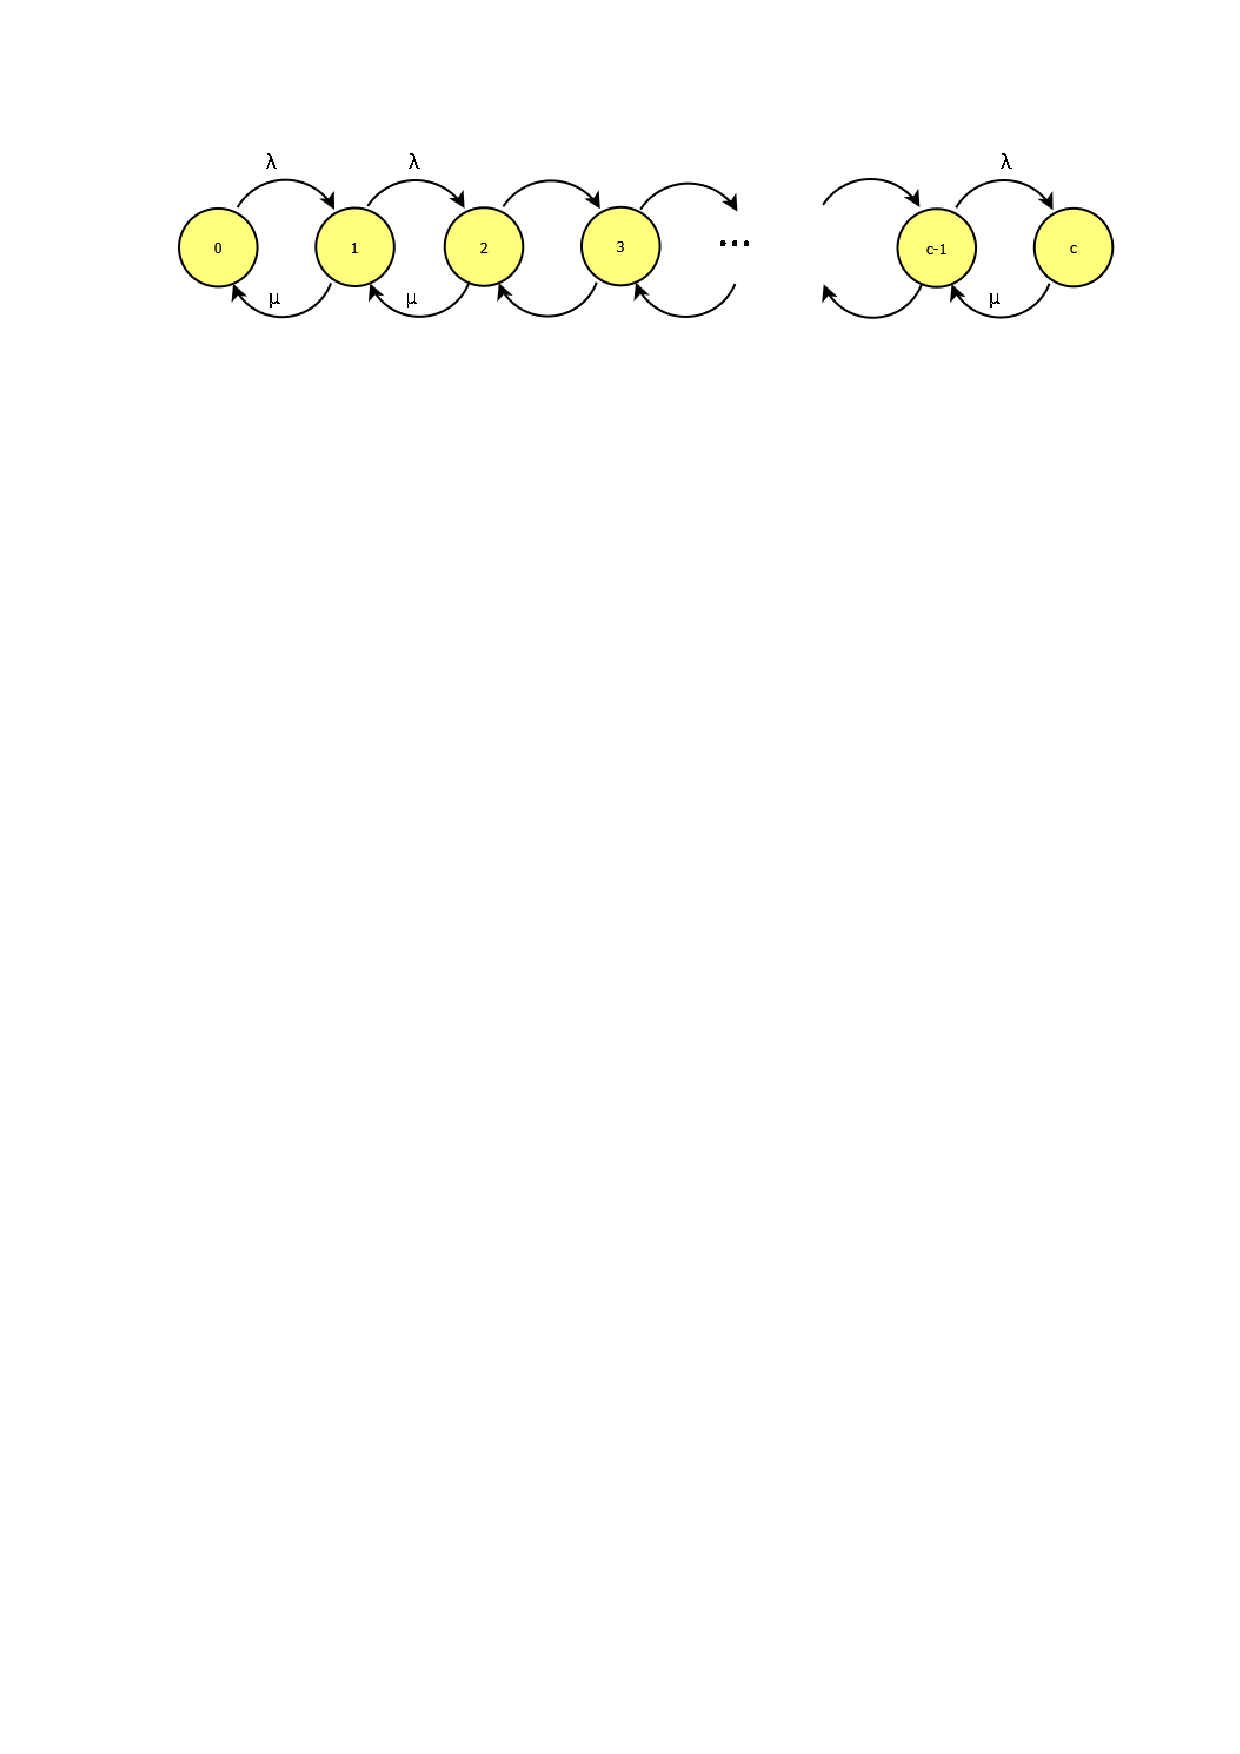
\includegraphics[trim = 10mm 220mm 10mm 25mm, clip,width=0.9\linewidth]{MMc}
			\end{center}
\end{frame}
\begin{frame}{M/M/1/c}

	Podemos modelar esta cola como un proceso de nacimiento-muerte con los siguientes parámetros: \pause
		$$\begin{array}{cc}
		\lambda_j=\lambda & (j=0,1,...,c-1)\\ \pause
		\lambda_c=0 & \\ \pause
		\mu_0=0 &  \\ \pause
		\mu_j=\mu &  (j=1,2,...,c)\\
		\end{array}$$
\end{frame}
\begin{frame}{M/M/1/c}
	Cuyas ecuaciones de balance serán: \pause
		$$\begin{array}{cc}
		\pi_0=\frac{1-\rho}{1-\rho^{c+1}} & \\ \pause
		\pi_j=\rho^j\pi_0 & (j=1,2,...,c)\\ \pause
		\pi_j=0 & (j=c+1,c+2,...)\\ \pause
		\end{array}$$
\end{frame}
\begin{frame}{M/M/1/c}
		\begin{block}{Cálculo de L}
	\begin{itemize}
		\item  Si $\rho=1$ tenemos que  \pause
		$$\begin{array}{cc}
		\pi_j=\frac{1}{c+1} & (j=0,1,...,c)\\ 
		
		L=\sum_{k=0}^{k=c}k\pi_k=\frac{c}{2}& \\
		\end{array}$$ \pause
		
		\item Si $\rho\neq1$ \pause
		\begin{center}
			$L=\sum_{k=0}^{c}k\frac{\rho^k (1-\rho)}{1-\rho^{c+1}}=...=\frac{\rho}{1-\rho}-\frac{(c+1)\rho^{c+1}}{1-\rho^{c+1}}$
		\end{center}
	
		\end{itemize}
	\end{block}
\end{frame}
\begin{frame}{M/M/1/c}
	
	\begin{itemize}
	\item 	$$L_s=1-\pi_=0$$  \pause
	\item  $$L_q=L-L_s=L-1+\pi_=0$$
	\end{itemize}
\end{frame}
\begin{frame}{M/M/1/c}
		\begin{block}{Cálculo de W}
	Como tiene capacidad finita no todas las personas podrán entrar en el sistema. El ratio de clientes que verdaderamente entrarán será:
	\pause
	\\
	 $\lambda-\lambda\pi_c=\lambda(1-\pi_c)$ \pause
	 \\
	 Usando las fórmulas de Little:
	\begin{itemize}
		\item $W=\frac{L}{\lambda(1-\pi_0}$ \pause
		\item $W_q=\frac{L_q}{\lambda(1-\pi_c)}$ \pause
		\item $W_s=\frac{1}{\mu}$ \pause
	\end{itemize}
\end{block}
\end{frame}

\begin{frame}
	\centering \LARGE \color{naranjaUCA} Modelo de cola M/M/s
			\begin{center}
				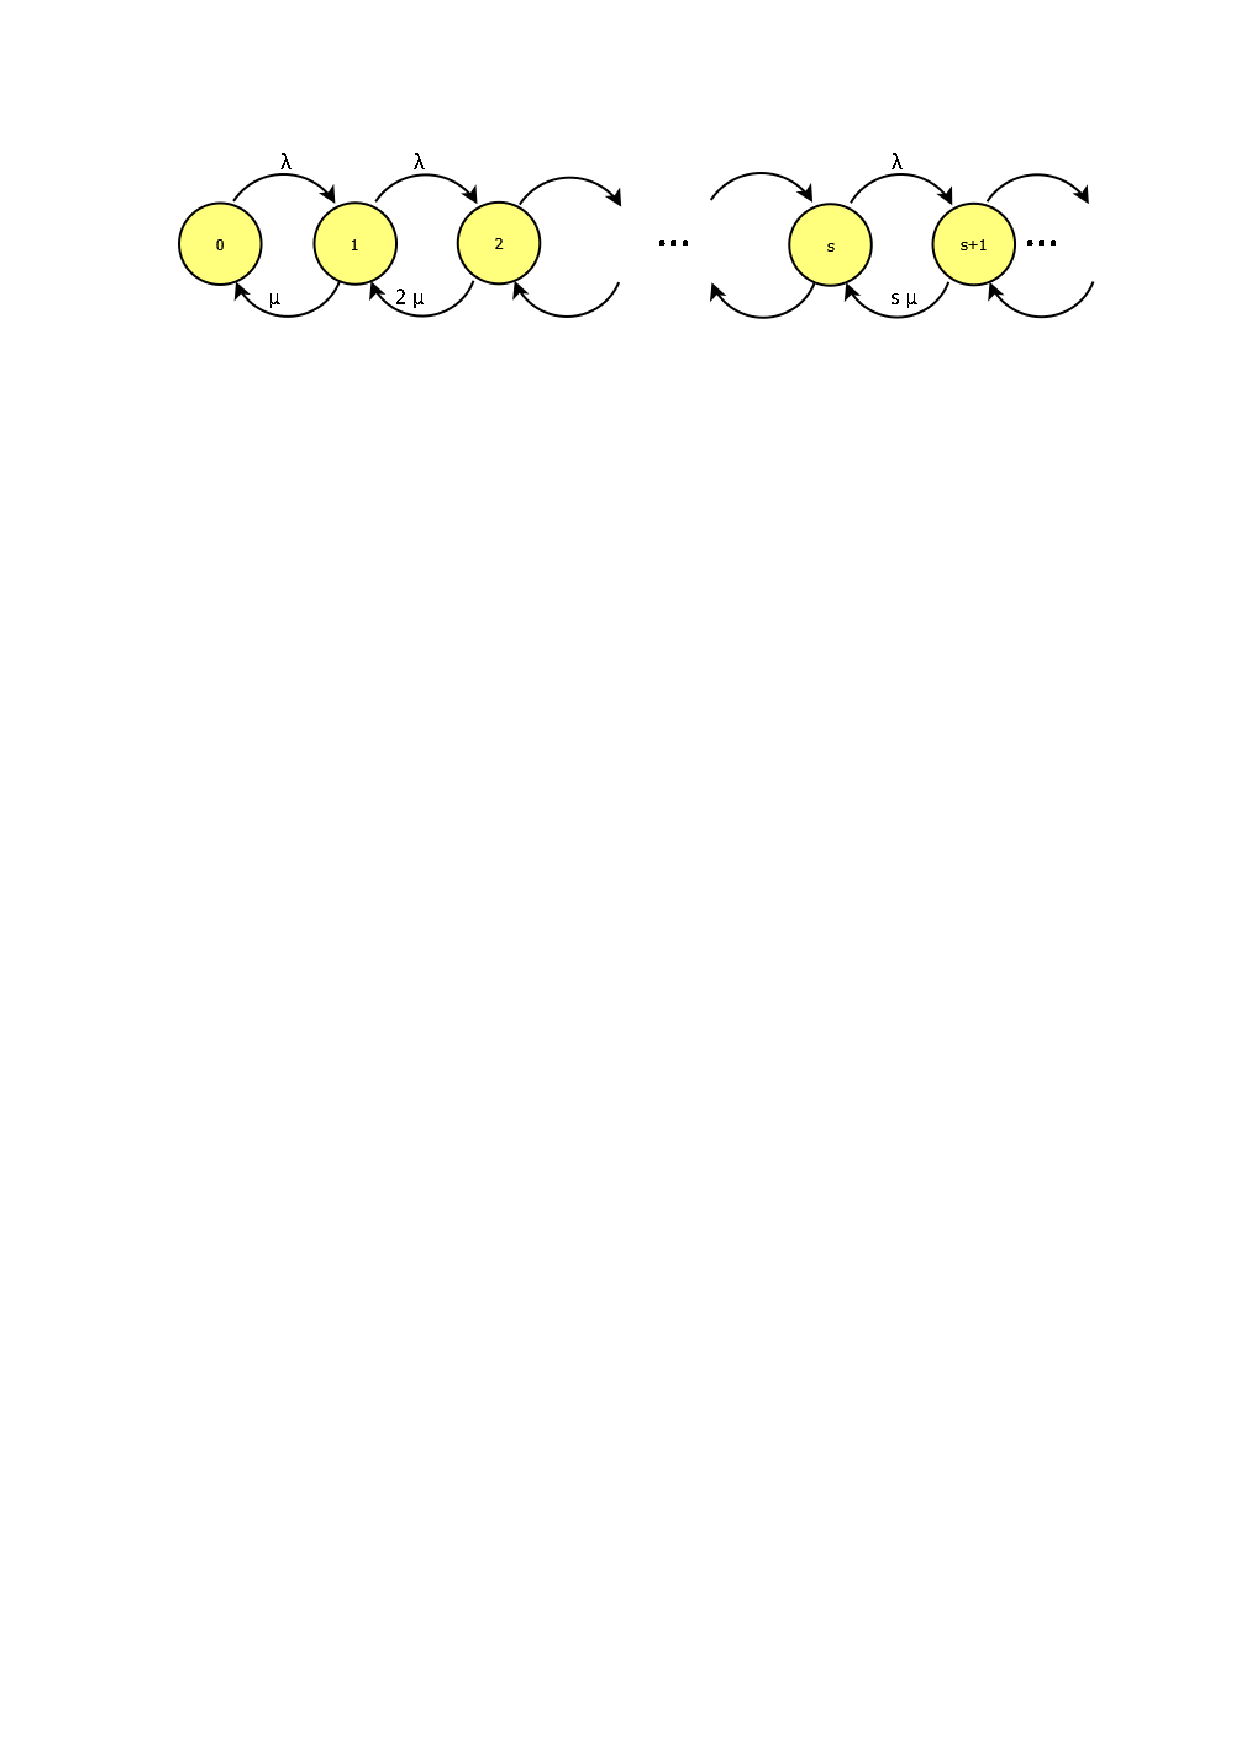
\includegraphics[trim = 10mm 220mm 10mm 25mm, clip,width=0.9\linewidth]{MMs}
			\end{center}
\end{frame}
\begin{frame}{M/M/s}
	Cuando en el sistema haya $j\leq s$ clientes, todos estar\'an siendo servidos. Cuando haya $j>s$, los que vayan llegando esperar\'an en la cola. \\
	\pause
	
	Este tipo de cola se puede modelizar como un proceso de nacimiento-muerte con los siguientes par\'ametros
	
	\pause
		$$\begin{array}{cc}
		\lambda_j=\lambda & (j=0,1,2,...)\\
		\mu_j=j\mu & (j=1,2,...,s)\\
		\mu_j=s\mu & (j=s+1,s+2,...)\\
		\end{array}$$
	\pause
	Definimos $\rho=\displaystyle\frac{\lambda}{s\mu}$.
	\\ 
	\pause
	Asumiendo $\rho\geq1$ 
\end{frame}

\begin{frame}{M/M/s}
	Usando las ecuaciones de equilibrio:
	$$\begin{array}{cc}
	\pi_0=\displaystyle\frac{1}{\displaystyle \sum_{t=0}^{t=s-1}\frac{(s\rho)^t}{t!}+\frac{(s\rho)s}{s!(1-\rho)}} & \\
	\pi_j=\displaystyle\frac{(s\rho)^j\pi_0}{j!} & (j=0,1,...,s)\\
	\pi_j=\displaystyle\frac{(s\rho)^j\pi_0}{s!s^{j-s}} & (j=s+1,s+2,...)\\
	\end{array}$$
	
	\pause
	La probabilidad de que todos los servidores est\'en ocupados, que viene dada por:
	$$P(j\geq s)=\sum_{k\geq s}^{}\pi_k=\frac{(s\rho)^s}{s!(1-\rho)}\pi_0$$
	$$L_q=\frac{P(j\geq s)\rho}{1-\rho}$$
\end{frame}

\begin{frame}{M/M/s}
	Por las fórmulas de Little obtenemos:		$$W_q=\frac{L_q}{\lambda}=\frac{P(j\geq s)}{s\mu-\lambda}$$
	\pause
	Una vez que el cliente est\'a en el servidor, como este sigue una distribuci\'on exponencial, tenemos que $W_s=\frac{1}{\mu}$ \pause
	$$L=L_q+L_s=L_q+\frac{\lambda}{\mu}$$
	\pause
	Por Little:
	$$W=\frac{L}{\lambda}=\frac{L_q}{\lambda}+\frac{1}{\mu}$$
\end{frame}

\begin{frame}
	\centering \LARGE \color{naranjaUCA} Modelo de cola M/G/1
\end{frame}
\begin{frame}{M/G/1}
Debido a que $G$ no es exponencial no podemos modelar este tipo de colas un proceso de nacimiento-muerte. \\ \pause
Utilizamos los resultados de Pollaczek y Khinchin para determinar $L_q$, $L$, $L_s$, $W_q$, $W$, $W_s$ \pause


\begin{equation}
L_q=\frac{\lambda^2 \sigma^2+\rho}{2(1-\rho)} ~ ~ ~ \rho=\frac{\lambda}{\mu}
\end{equation}
Como $W_s=\displaystyle\frac{1}{\mu}$, por Little tenemos:
$L_s=\lambda\left(\displaystyle\frac{1}{\mu}\right)=\rho$. Como $L=L_s+L_q$ obtenemos que
\begin{equation}
L=L_q+\rho
\end{equation}


\end{frame}

\begin{frame}{M/G/1}
Nuevamente de las fórmulas de Little tenemos

$$
W_q=\frac{L_q}{\lambda}$$
$$
W=W_q+\frac{1}{\mu}
$$

\end{frame}

\begin{frame}
	\centering \LARGE \color{naranjaUCA} Ruegos y preguntas
\end{frame}
\begin{frame}
	\begin{block}{Descargar trabajo completo}
		\begin{itemize}
			\item \textbf{Código látex: } goo.gl/Vdq8bV
			\item \textbf{PDF compilado: } goo.gl/kELghg
		\end{itemize}
	\end{block}
	\begin{block}{Descargar presentación}
			\begin{itemize}
				\item \textbf{Código látex: } goo.gl/V5xIbW
				\item \textbf{PDF compilado: } goo.gl/aCvjil
			\end{itemize}
	\end{block}
\end{frame}

\begin{frame}
	\centering \LARGE \color{naranjaUCA} Autores
\end{frame}
\begin{frame}
\begin{block}{Referencia}
	\begin{enumerate}
		\item Investigación de operaciones - Wayne L. Winston.
		\item Applied Stochastics Processes - Mario Lefebvre
		\item Apuntes del curso 'Procesos estocásticos y series temporales' - Miguel Ángel Sordo Díaz
	\end{enumerate}
\end{block}
\begin{block}{Autores}
	\begin{itemize}
		\item José Carlos García Ortega
		\item Álvaro Ramírez Moreno
		\item Juan Manuel Pérez Sánchez
		\item Marina Gandullo Escobar
	\end{itemize}
\end{block}
\end{frame}

\end{document}
